\documentclass{llncs}

\usepackage[english]{babel}
\usepackage[utf8x]{inputenc}
%\usepackage{amsmath}
\usepackage{graphicx}

\sloppy

\title{Sentiment Analysis and Visualization using UIMA and Solr}
\author{Carlos Rodríguez-Penagos, David García Narbona, Guillem Massó Sanabre, Jens Grivolla, Joan Codina Filbá}
\institute{Barcelona Media Innovation Centre}

\begin{document}
\maketitle

\begin{abstract}
In this paper we present an overview of a UIMA-based system for Sentiment Analysis in hotel customer reviews. It extracts object-opinion/attribute-polarity triples using a variety of UIMA modules, some of which are adapted from freely available open source components and others developed fully in-house. A Solr based graphical interface is used to explore and visualize the collection of reviews and the opinions expressed in them.
\end{abstract}

\section{Introduction}

With the continuing growth of Social Media such as Twitter, Facebook, and many others, both in terms of volume of content produced daily by users, and in terms of the impact it can have for reputation and decision making (buying, travelling, ...) there is a strong commercial need (and social interest) to efficiently analyze those vast amounts of mostly unstructured information and extract summarized knowledge, while also being able to explore and navigate the content.

We present here a prototype system for analyzing customer reviews of hotels, detecting what people talk about and what opinions they express. The literature agrees on two main approaches for classifying opinion expressions: using supervised learning methods and applying dictionary/rule-based knowledge (see \cite{liu_sentiment_2012} for an overview). The choice of content to be processed also determines what kind of technique yields better results, since longer, more textured text accomodates deeper lingüistic analyses including, for example, dependency parsing (see, for example, the use of Machine Learning informed with linguistic analyses in \cite{wilson_recognizing_2010}) while shorter, noisy messages, such as those from Twitter microblogs can be tackled with more superficial processing that is strengthened by massive training data and extensive lexical resources (as shown in previous work from some of the authors: \cite{rodriguez-penagos_fbm:_2013,chenlo_fbm-yahoo!_2012}. Each of them on its own has been used in workable systems\cite{zhang_combining_2011} and a principled combination of both of them can yield good results on noisy data, since generally one (dictionaries/rules) offers good precision while the other (ML) is able to discover unseen examples and thus enhances recall. In the case at hand, the processing at the level of individual reviews is done using UIMA with a variety of analysis engines using both stochastic and symbolic approaches; the summary of the results, visualization and exploration interface is based on Solr.

\section{Extraction of Opinionated Units}

The prototype presented here focuses on the extraction of customer opinions from full-text unstructured reviews, provided by the users of a big customer review site. We identified as the object of interest for our analysis what we call "opinionated units". These OUs consist in:
\begin{itemize}
\item the object of the opinion, i.e. the thing that is being commented on, which we call \emph{Target}.
\item the opinion expression, i.e. the words or sentence fragments that represent what is being said about the target, which we call \emph{Cues}.
\item the \emph{polarity} of the opinion, as it relates to the target.
\end{itemize}

Our system proceeds by first detecting possible opinion Targets and possible Cues in the review text. These Target and Cue candidates are then correlated to form Opinionated Units using relevant paths of the  syntactic dependencies graph that link the two together. Finally, the polarity of the opinionated unit is established using an \emph{apriori} polarity taken from the Cue (possibly dependent on the type of target) and taking into account quantifiers and negations that appear in the context of the opinionated unit.

For the detection of the possible targets and cues that anchor the OUs, we relied on a JNET annotator that uses Conditional Random Fields over richly annotated vectors (POS, NER, polar words, NP chunks, etc.), and that was trained with a manually annotated corpus of similar customer reviews.\footnote{On evaluating this process, we allowed for partial overlap (e.g. "The room" and "room" counted as equally correct answers), and we obtained models that had F1 of 0.69 for  Targets only, 0.54 for Cues and a combined Target/Cue identification model that provided an F1 of 0.62, with a top precision of 0.84 for the Cue only model and a top coverage (or recall) of 0.63 for Target-only models.} We used this supervised approach since the hotel review domain is pretty regular inasmuch the kinds of things and features people comment on, but we wanted to leave open the possibility to discover items and concepts outside a closed list.


\subsection{Recognizing Opinionated Units and their polarity}

In order to detect candidate opinion-bearing linguistic structures we parsed the sentences with the DeSR dependency parser\cite{attardi_multilingual_2007}. We looked for possible paths in the graph linking Cues to Targets, as show in Figure \ref{fig:GRAFO}, where the Target "la habitación" (the room) is qualified by "pequeña" (small) and the Target "el desayuno" (breakfast) is being described as "with room for improvement".

\begin{figure}[ht]
\centering
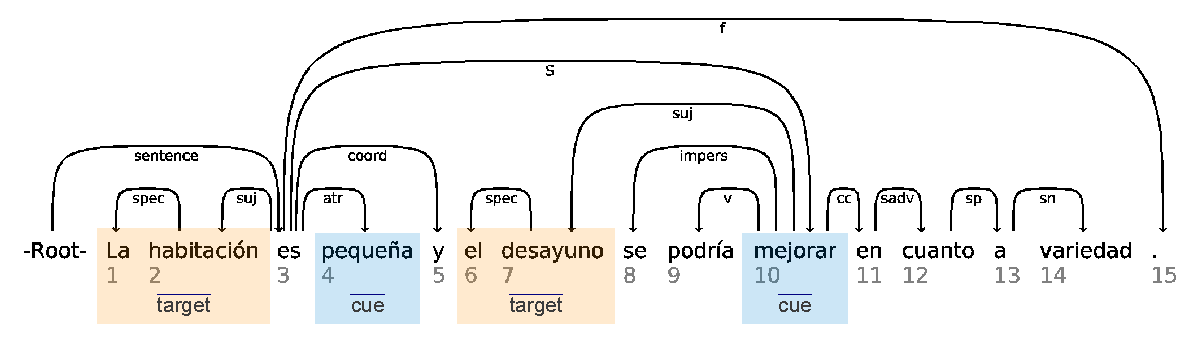
\includegraphics[width=9cm]{grafo.pdf}
\caption{Opinionated Units in the dependency graph}
\label{fig:GRAFO}
\end{figure}

We identified both correct and wrong paths between Targets and Cues in annotated documents and analysed them. This allowed us to extract relevant patterns, and individualize opinionated units even if they were expressed in the same phrase. The most important patterns are structures of linking verbs and name-adjective relations, but there are prepositional phrases, adverbial phrases and subject-verb relations as well. All the relevant paths can be represented by a limited number or regular expressions, which are used to correlate Targets and Cues of the same OU. This approach maximized precision at the expense of recall, focusing further analyses only in semantically relevant fragments, as identified through Targets and Cues.

We used different strategies and tools to detect the possible polarity of an Opinionated Unit, since each one has both advantages and weaknesses. A first strategy is to assign polarities to Cues, and then expand this polarity to the Opinionated Unit, using an aproach based on the words sequence (Conditional Random Fields). A second strategy uses Support Vector Machines on a "bag of features" that includes words, polar words and their polarity, negations, and quantifiers to build a feature vector used for training and classification. 
\begin{figure}[ht!]
\centering
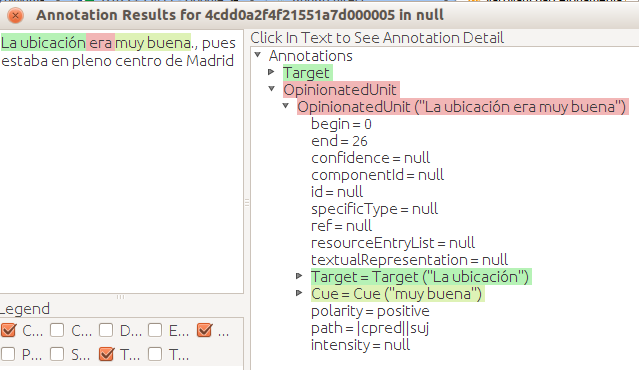
\includegraphics[width=6cm]{bookingOU.png}
\caption{Type representation of the Opinionated Unit visualized with the Annotation Viewer}
\label{fig:xmi}
\end{figure}
After statistical models have been applied, we also used heuristics that combined those polarities with the polarities of key words (detected using dictionaries) in the context of the OUs, in order to assign a final polarity to the Opinionated Unit. Our UIMA type for Opinionated Units representing the Target-Polarity-Cue triplet has pointers to corresponding Targets and Cues from the relevant dependency graph, as well as the span and ultimate polarity of the complete object covered by it, as shown in Figure \ref{fig:xmi} for the text "The location [Target] was very good [Cue]".

\begin{figure}[ht!]
\centering
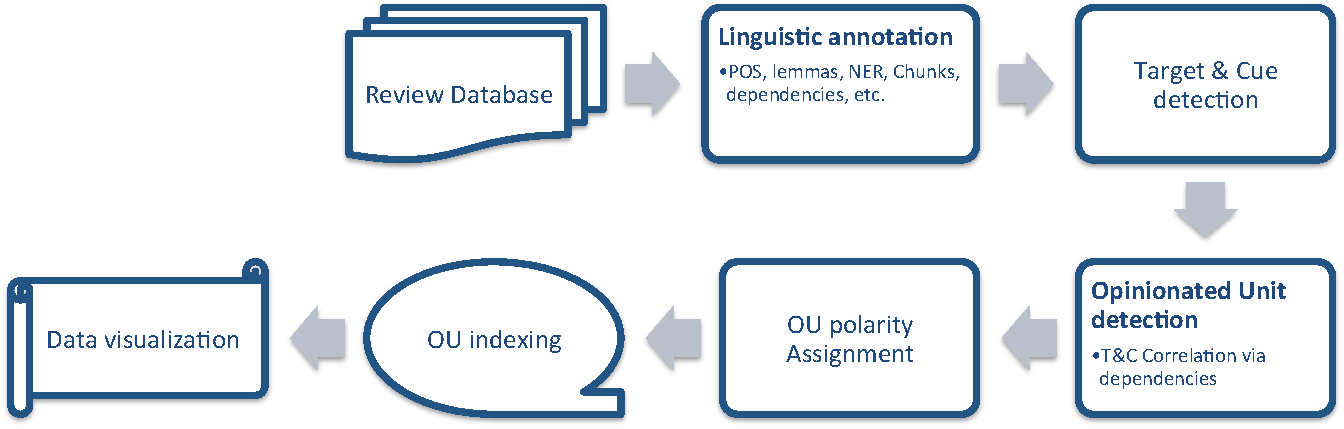
\includegraphics[width=7cm]{pipelineOverview.pdf}
\caption{System overview}
\label{fig:pipeline}
\end{figure}

\section{Architecture and Implementation}

This section describes all UIMA modules used in the prototype, as implemented in Figure \ref{fig:pipeline}. Some of them are existing open source components, some are adaptations, and some are our own custom developments. We have been publishing our work on Github and will continue doing so as far as possible.\footnote{See \url{https://github.com/BarcelonaMedia-ViL/}}

\subsubsection{UIMA Collection Tools}

This prototype is designed to work on a static document collection, previously loaded into a MySQL database (including the review text as well as associated metadata). 
 UIMA Collection Tools\footnote{The UIMA Collection tools have been developed at Barcelona Media, some of them based on the example Collection Readers and CAS Consumers provided with the UIMA distribution. They are published under the Apache License at \url{https://github.com/BarcelonaMedia-ViL/uima-collection-tools}.} is an \emph{ecosystem} of tools for allowing UIMA pipelines to store and retrieve data from database systems, such as MySQL.
Plain text documents can be retrieved from a database, XMI documents can be retrieved from and stored in a database either compressed or uncompressed, features can be extracted into a database table, and annotations within database-stored XMI blobs can be visualized the same way as the standard AnnotationViewer does for XMI files.

\begin{itemize}
\item \emph{DBCollectionReader} is a UIMA collection reader which retrieves plain text documents stored in a MySQL database. Database connection parameters as well as SQL query have to be specified in the component descriptor. It is derived from the FileSystemCollectionReader.

\item \emph{SolrCollectionReader} is equivalent to DBCollectionReader, but using a Solr index as the document source.

\item \emph{DBXMICollectionReader} is a UIMA collection reader that retrieves XMI documents stored in a MySQL database. DBXMICollectionReader is also prepared to read compressed XMI documents by means of ZLIB compression. This option can be set in the descriptor file.

\item \emph{DBAnnotationsCASConsumer} is a CAS consumer which stores values of the features specified in the component descriptor file in a MySQL database table. Each table row corresponds to the annotation defined as the \emph{splitting annotation}, e.g. if Sentence annotation has been defined as the \emph{splitting annotation}, each table row will correspond to a Sentence, and this row will contain features of the Sentence annotation and/or features of annotations covered by the Sentence annotation.

\item \emph{DBXMICASConsumer} is a CAS consumer that persists XMI documents in a database. DBXMICASConsumer is also prepared to store compressed XMI documents by means of ZLIB compression. 

\item \emph{DBAnnotationViewer} is a modification of the Annotation Viewer, and allows reading XMI files directly from a MySQL database without needing to extract them first.
\end{itemize}

\subsubsection{OpenNLP}

We use OpenNLP\footnote{\url{http://opennlp.apache.org/}} with the standard UIMA wrappers for our base pipeline, including Sentence Detector, Tokenizer, and POS Tagger, using our own trained models for Spanish.

\subsubsection{Lemmatizer}

We apply Lemmatization using a large dictionary developed in-house. All candidate lemmas are first added to the CAS using ConceptMapper\footnote{\url{http://uima.apache.org/sandbox.html\#concept.mapper.annotator}} but a second custom component selects the right one using the POS tag.

\subsubsection{JNET}

For ML-based detection of Targets and Cues we use JNET\footnote{\url{http://www.julielab.de/Resources/Software/NLP\_Tools.html}} (the Julielab Named Entity Tagger), which is based on Conditional Random Fields (CRF). It detects token sequences that belong to certain classes, taking into account  a variety of features associated with each token (such as the surface form, lemma, POS tag, surface features such as capitalization, etc.) as well as its context of preceeding and successive tokens. While originally intended for Named Entity Recognition, we trained JNET with our own manually annotated corpus.

Compared to the original JNET as released by JulieLab we introduced a series of changes, most importantly making it type system independent by taking all input and output types and features as parameters, and fixing some bugs that were triggered when using a larger amount of token features. We expect to release our changes soon, but are still looking into the question of licensing, to comply with JNET's original license.

\subsubsection{DeSR}

We developed a UIMA wrapper for the DeSR dependency parser\footnote{\url{https://sites.google.com/site/desrparser/}}. The parser creates dependency annotations based on previously generated sentence, token and POStag annotations. It is available at \url{https://github.com/BarcelonaMedia-ViL/desr-uima}. The UIMA DeSR analysis engine is a UIMA C++ annotator, developed using the C++ SDK provided by UIMA. It translates between the format required by the DeSR parser shared library and the UIMA CAS format. The mapping between UIMA types and features and the features used internally by DeSR is configurable in the annotator descriptor.

\subsubsection{DependencyTreeWalker}

This is a Pythonnator-based analysis engine for wrapping the DependencyGraph Python module (both developed in-house). This allows us to work easily with the dependency graph generated by DeSR in order to e.g. determine and validate the path between two given UIMA annotations.

\subsubsection{Weka Wrapper}

We used the Mayo Weka/UIMA Integration (MAWUI\footnote{\url{http://informatics.mayo.edu/text/index.php?page=weka}}), as a basis for the machine learning tools. The version we use is adapted to newer versions of UIMA and made much more configurable. MAWUI generates a single vector for each document, that is used to classify it as a whole. In our case, a document can contain several Opinionated Units that need to be classified. For this reason the Weka Wrapper was adapted to be able to deal with all the annotations of a given type inside a document (or collection when generating the training data).

\section{Visualization}

Beyond being able to extract and classify the opinions, users need an interface that allows them to access and explore the data. They need to know which are the Targets or its features that are being addressed by the opinions and what is being said about them, and this has to be shown in an aggregated way, with drill-down capabilities, so that the end user has a clear view of the contents of hundreds or thousands of opinions.

UIMA does not provide tools to deal with collections of documents, and we use Solr, a Lucene based indexing tool, to index the Opinionated Units. Through the use of Solr's faceting and pivot utilities we are able to graphically summarize thousands of opinions. Special charts have been dconstructed in order to allow not only to represent the data but also to select subsets of opinions and summarize and compare them. For example, we can compare the global user's opinions with the opinions about a single hotels or the hotels in a specific area. 

To index the data we needed the linguistic information, but also the metadata associated with the opinion, which is located in databases and is not processed with UIMA. For this reason we import the data to Solr in two steps. In a first step we generate from UIMA a table with the data that we then import to Solr together with the metadata.

\subsection{Indexing Opinionated Units}

To index the Opinionated Units we use the DBAnnotationsCASConsumer component. We generate a register for each OU, containing: the Target, the Cue, the text span, the polar words, their polarity, the polarity of the cue, and the polarity of the Opinionated Unit. Cues and targets are grouped in single tokens by means of underscoring.

We use the the DataImportHandler from Solr in order to import the data from the database. To do it, a query combines the opinionated unit information with the one related with the hotel or the user who writes the opinion. Cues are indexed twice, once all merged and later in different fields depending on the opinion's polarity, making it easy to retrieve just the positive or negative opinion markers. We selected this option because it is a bit faster, more flexible and reliable than the other ones: when indexing directly from UIMA we have problems in adding all the desired metadata, and if we call UIMA from Solr (or Lucene) then it is difficult to have a general framework that splits a single document into several Opinionated Units.

AJAX-Solr (https://github.com/evolvingweb/ajax-solr) is a JavaScript library for creating user interfaces to Apache Solr. This library works with facets. Faceting is a capability of Solr that allows to have a fast statistic of the most frequent terms in each field, after performing a query. Since version 4.0 Solr also has pivots that combine the facets from two or more different fields. We adapted AJAX-Solr to work with pivots and wrote a series of widgets to visualize them. Our own extensions to AJAX-Solr are also published on github\footnote{\url{https://github.com/BarcelonaMedia-ViL/ajax-solr}}.

By means of clicking the different facets that appear on the widgets, the user can build a query that restricts the set of opinions to summarize. These opinions are then summarized by showing the most frequent terms they contain, or the most differentiating ones\footnote{The most differentiating ones being those terms that are frequent in the current subset but that are less frequent in the general one}. Figure \ref{fig:solr} shows the pivot result in text and force diagram formats. It shows the relationship between Targets, and positive and negative Cues. In the textual representation, the relationships are not shown directly but scaled to magnify the most discriminative ones. 

\begin{figure}[ht!]
\centering
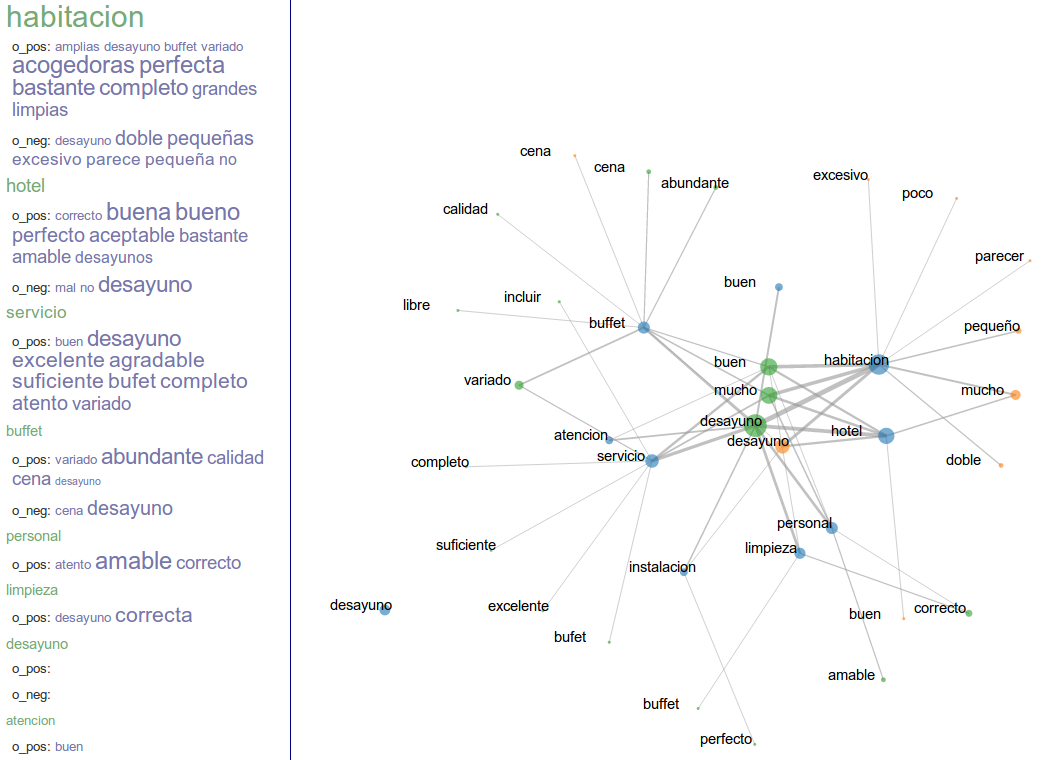
\includegraphics[width=5cm]{solr_visualization.png}
\caption{Visualization of Cue and Target correlations across the whole corpus} 
\label{fig:solr}
\end{figure}

\section{Conclusion}

The combination of UIMA and Solr has allowed us to to develop a very flexible platform that makes it easy to integrate and combine processing modules from a variety of sources and in a variety of programming languages, as well as navigate and visualize the results easily and efficiently.

In our evaluations with 700 OUs manually annotated by 3 independent reviewers, there was an agreement on the correctness of the OU identified by the system of 92\%, while the polarity assigned was found to be correct an average of 70\%.

We found many useful UIMA components to be available as open source, and encountered few compatibility issues (other than adapting some components to be type system independent). Solr provides us with a very flexible platform to access large document collections, and in combination with UIMA allows us to explore even complex hidden relationships within those collections.

One of our main objectives was to make all modules configurable and reusable, inasmuch as Sentiment Analysis in general requires tweaking to adapt to domain and genre, but this generalization often requires considerable effort. We found the different open source communities to be very receptive, and we try to participate by publishing our own contributions under permissive licenses that make them easy for others to adopt and use.

\section{Thanks}
This work has been partially funded by the Spanish
Government project Holopedia, TIN2010-21128-
C02-02, and the CENIT program project Social Media,
CEN-20101037.

\bibliographystyle{plain}
\bibliography{gscl2013}

\end{document}